\section{Datasets}
\label{sec:datasets}

The pipeline and its offensive extension produce two polarizing datasets.

\subsection{Defensive instruction dataset}

The defensive dataset (\datasetname) is the direct output of the
pipeline. Table~\ref{tab:dataset-basic} summarizes its scale: it is fully
deduplicated in a three-turn
\texttt{system}$\to$\texttt{user}$\to$\texttt{assistant} chat format.

% AUTO-GENERATED by gen_tables.py -- do not edit
\begin{table}[t]
\centering
\small
\caption{Defensive instruction dataset: basic statistics.}
\label{tab:dataset-basic}
\begin{tabular}{lr}
\hline
\textbf{Metric} & \textbf{Value} \\
\hline
Total samples & 1,416 \\
Unique samples & 1,416 \\
Duplicate rate & 0.00\% \\
File size (MB) & 7.97 \\
Total tokens & 1,661,580 \\
Vocabulary size & 18,781 \\
Code-bearing samples & 11.5\% \\
\hline
\end{tabular}
\end{table}


Text-length statistics (Table~\ref{tab:dataset-text}) reveal polarizing
information: a large mass of very short items sits alongside long technical
answers, so the mean token count far exceeds the median. This is consistent
with the source mix (advisory records mixed with extended
explanations) and with the low readability scores typical of security prose.

% AUTO-GENERATED by gen_tables.py -- do not edit
\begin{table}[t]
\centering
\small
\caption{Defensive dataset text-length statistics per sample. The large mean/median gap reflects a strongly bimodal distribution (short prompts, long technical answers).}
\label{tab:dataset-text}
\begin{tabular}{lrrrr}
\hline
\textbf{Unit} & \textbf{Mean} & \textbf{Median} & \textbf{Std} & \textbf{P95} \\
\hline
Tokens & 391.1 & 32.0 & 558.4 & 1413 \\
Words & 265.6 & 24.0 & 372.6 & 939 \\
Characters & 1924.4 & 198.0 & 2682.2 & 6753 \\
\hline
\end{tabular}
\end{table}


Domain coverage (Table~\ref{tab:dataset-domains}, Figure~\ref{fig:domains}),
computed by overlapping keyword matching, is broad across defensive, forensic,
threat intelligence, vulnerability, and attack analysis content, but thins out
for cryptography and drops sharply for compliance ($6.7\%$), the clearest
coverage gap and a natural target for future collection.

% AUTO-GENERATED by gen_tables.py -- do not edit
\begin{table}[t]
\centering
\small
\caption{Domain coverage of the defensive dataset (keyword-based, overlapping). Compliance is the clear coverage gap.}
\label{tab:dataset-domains}
\begin{tabular}{lr}
\hline
\textbf{Domain} & \textbf{Coverage} \\
\hline
Defense & 100.0\% \\
Forensics & 95.3\% \\
Threat intel & 92.9\% \\
Vulnerability & 89.5\% \\
Attack & 89.1\% \\
Network & 78.0\% \\
Cryptography & 31.6\% \\
Compliance & 6.7\% \\
\hline
\end{tabular}
\end{table}


\begin{figure}[t]
  \centering
  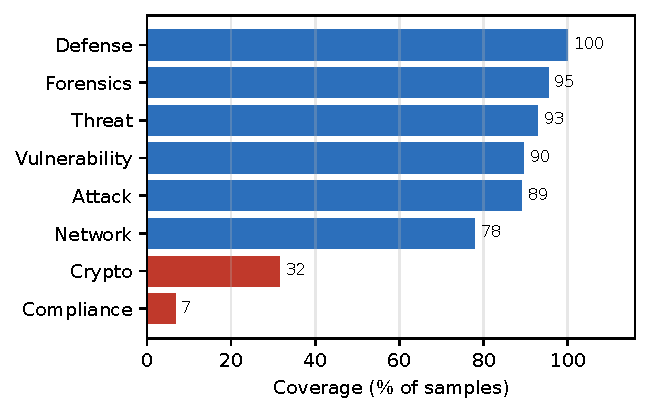
\includegraphics[width=\columnwidth]{fig_domains.pdf}
  \caption{Domain coverage of the defensive dataset. Compliance
  (highlighted) is the dominant coverage gap.}
  \label{fig:domains}
\end{figure}

\subsection{Offensive exploitation dataset}

The offensive branch (\offensivename) departs from the defensive pipeline in
purpose and in method. It takes the public
\texttt{CyberNative/\allowbreak Code\_\allowbreak Vulnerability\_\allowbreak Security\_\allowbreak DPO}
corpus~\cite{cybernative} and, for each vulnerable code sample, uses an
abliterated local model to synthesize an assistant answer that
identifies the vulnerability and provides exploitation guidance,
structured as an audit summary, findings, exploitation steps, and payload
examples. Table~\ref{tab:offensive-sizes} gives the split sizes; a
metadata file records per-record provenance (source dataset, row index,
language, and vulnerability class).

% AUTO-GENERATED by gen_tables.py -- do not edit
\begin{table}[t]
\centering
\small
\caption{Offensive exploitation SFT dataset, synthesized by an abliterated model over the public CyberNative Code\_Vulnerability\_Security\_DPO corpus.}
\label{tab:offensive-sizes}
\begin{tabular}{lr}
\hline
\textbf{Split} & \textbf{Records} \\
\hline
Train & 4,656 \\
Validation & 465 \\
Test & 419 \\
\textbf{Total} & \textbf{5,540} \\
\hline
\end{tabular}
\end{table}


Two design choices make this branch the ethically load-bearing part of the
work: it \emph{omits} the security-alignment stage the defensive pipeline is
meant to include, and it uses a de-aligned generator so the synthesis does not
refuse. (\S\ref{sec:dualuse}).

\subsection{Preference data}

A third, defensive preference dataset is derived from the same CyberNative
source for DPO/ORPO training: the \emph{chosen} response is a safe rewrite of
the vulnerable code and the \emph{rejected} response retains the
vulnerability.
